\documentclass{article}\usepackage[]{graphicx}\usepackage[]{color}
%% maxwidth is the original width if it is less than linewidth
%% otherwise use linewidth (to make sure the graphics do not exceed the margin)
\makeatletter
\def\maxwidth{ %
  \ifdim\Gin@nat@width>\linewidth
    \linewidth
  \else
    \Gin@nat@width
  \fi
}
\makeatother

\definecolor{fgcolor}{rgb}{0.345, 0.345, 0.345}
\newcommand{\hlnum}[1]{\textcolor[rgb]{0.686,0.059,0.569}{#1}}%
\newcommand{\hlstr}[1]{\textcolor[rgb]{0.192,0.494,0.8}{#1}}%
\newcommand{\hlcom}[1]{\textcolor[rgb]{0.678,0.584,0.686}{\textit{#1}}}%
\newcommand{\hlopt}[1]{\textcolor[rgb]{0,0,0}{#1}}%
\newcommand{\hlstd}[1]{\textcolor[rgb]{0.345,0.345,0.345}{#1}}%
\newcommand{\hlkwa}[1]{\textcolor[rgb]{0.161,0.373,0.58}{\textbf{#1}}}%
\newcommand{\hlkwb}[1]{\textcolor[rgb]{0.69,0.353,0.396}{#1}}%
\newcommand{\hlkwc}[1]{\textcolor[rgb]{0.333,0.667,0.333}{#1}}%
\newcommand{\hlkwd}[1]{\textcolor[rgb]{0.737,0.353,0.396}{\textbf{#1}}}%
\let\hlipl\hlkwb

\usepackage{framed}
\makeatletter
\newenvironment{kframe}{%
 \def\at@end@of@kframe{}%
 \ifinner\ifhmode%
  \def\at@end@of@kframe{\end{minipage}}%
  \begin{minipage}{\columnwidth}%
 \fi\fi%
 \def\FrameCommand##1{\hskip\@totalleftmargin \hskip-\fboxsep
 \colorbox{shadecolor}{##1}\hskip-\fboxsep
     % There is no \\@totalrightmargin, so:
     \hskip-\linewidth \hskip-\@totalleftmargin \hskip\columnwidth}%
 \MakeFramed {\advance\hsize-\width
   \@totalleftmargin\z@ \linewidth\hsize
   \@setminipage}}%
 {\par\unskip\endMakeFramed%
 \at@end@of@kframe}
\makeatother

\definecolor{shadecolor}{rgb}{.97, .97, .97}
\definecolor{messagecolor}{rgb}{0, 0, 0}
\definecolor{warningcolor}{rgb}{1, 0, 1}
\definecolor{errorcolor}{rgb}{1, 0, 0}
\newenvironment{knitrout}{}{} % an empty environment to be redefined in TeX

\usepackage{alltt}
\IfFileExists{upquote.sty}{\usepackage{upquote}}{}
\begin{document}

\title{Frankenstein Wordcloud}
\author{William Taylor Bickelmann}
\maketitle

\begin{abstract}
This PDF will contain a wordcloud and title of the book 'Alice in Wonderland' by Lewis Carroll.

\end{abstract}

\textit{Alice in Wonderland}

\section{packages}
This section will contain the packages which will then be used to load 'Alice in Wonderland', manipulate string and form wordclouds.

\begin{knitrout}
\definecolor{shadecolor}{rgb}{0.969, 0.969, 0.969}\color{fgcolor}\begin{kframe}
\begin{alltt}
\hlstd{package}\hlkwb{<-}\hlkwd{c}\hlstd{(}\hlstr{'dplyr'}\hlstd{)}
\hlkwd{library}\hlstd{(tidytext)}
\hlkwd{library}\hlstd{(tm)}
\end{alltt}


{\ttfamily\noindent\itshape\color{messagecolor}{\#\# Loading required package: NLP}}\begin{alltt}
\hlkwd{library}\hlstd{(wordcloud)}
\end{alltt}


{\ttfamily\noindent\itshape\color{messagecolor}{\#\# Loading required package: RColorBrewer}}\begin{alltt}
\hlkwd{library}\hlstd{(stringr)}
\hlkwd{library}\hlstd{(dplyr)}
\end{alltt}


{\ttfamily\noindent\itshape\color{messagecolor}{\#\# \\\#\# Attaching package: 'dplyr'}}

{\ttfamily\noindent\itshape\color{messagecolor}{\#\# The following objects are masked from 'package:stats':\\\#\# \\\#\#\ \ \ \  filter, lag}}

{\ttfamily\noindent\itshape\color{messagecolor}{\#\# The following objects are masked from 'package:base':\\\#\# \\\#\#\ \ \ \  intersect, setdiff, setequal, union}}\begin{alltt}
\hlkwd{library}\hlstd{(knitr)}
\hlkwd{library}\hlstd{(gutenbergr)}
\end{alltt}
\end{kframe}
\end{knitrout}

The first step is to determine the id of Alice in Wonderland:

\begin{knitrout}
\definecolor{shadecolor}{rgb}{0.969, 0.969, 0.969}\color{fgcolor}\begin{kframe}
\begin{alltt}
\hlkwd{gutenberg_works}\hlstd{()}\hlopt
  \hlkwd{select}\hlstd{(gutenberg_id,title,author)}\hlopt
  \hlkwd{filter}\hlstd{(author}\hlopt{==}\hlstr{'Carroll, Lewis'}\hlstd{)}
\end{alltt}
\begin{verbatim}
## # A tibble: 18 x 3
##    gutenberg_id
##           <int>
##  1           11
##  2           12
##  3           13
##  4          620
##  5          651
##  6         4763
##  7        19002
##  8        28696
##  9        28885
## 10        29042
## 11        29888
## 12        33582
## 13        35497
## 14        35535
## 15        36308
## 16        38065
## 17        48630
## 18        48795
## # ... with 2 more variables: title <chr>, author <chr>
\end{verbatim}
\end{kframe}
\end{knitrout}

\noindent In the resulting tibble from the code above, one can pick out the id of Alice; 11.

\section{Chapter 1}

Here I want to isolate the 'chapter 1' block of text
\begin{knitrout}
\definecolor{shadecolor}{rgb}{0.969, 0.969, 0.969}\color{fgcolor}\begin{kframe}
\begin{alltt}
\hlkwd{library}\hlstd{(stringr)}
\hlstd{df} \hlkwb{<-} \hlkwd{gutenberg_download}\hlstd{(}\hlnum{11}\hlstd{)}
\end{alltt}


{\ttfamily\noindent\itshape\color{messagecolor}{\#\# Determining mirror for Project Gutenberg from http://www.gutenberg.org/robot/harvest}}

{\ttfamily\noindent\itshape\color{messagecolor}{\#\# Using mirror http://aleph.gutenberg.org}}\begin{alltt}
\hlkwd{head}\hlstd{(df[}\hlkwd{str_detect}\hlstd{(df}\hlopt{$}\hlstd{text,} \hlstr{'^CHAPTER'}\hlstd{),],}\hlkwc{n}\hlstd{=}\hlnum{1}\hlstd{)}\hlopt{$}\hlstd{text}
\end{alltt}
\begin{verbatim}
## [1] "CHAPTER I. Down the Rabbit-Hole"
\end{verbatim}
\end{kframe}
\end{knitrout}


\section{The Wordcloud}
Next the wordcloud package will be used to form a wordcloud
\begin{knitrout}
\definecolor{shadecolor}{rgb}{0.969, 0.969, 0.969}\color{fgcolor}\begin{kframe}
\begin{alltt}
\hlstd{words_df}\hlkwb{<-}\hlstd{df}\hlopt
  \hlkwd{unnest_tokens}\hlstd{(word,text)}

\hlstd{words_df}
\end{alltt}
\begin{verbatim}
## # A tibble: 26,694 x 2
##    gutenberg_id       word
##           <int>      <chr>
##  1           11    alice's
##  2           11 adventures
##  3           11         in
##  4           11 wonderland
##  5           11      lewis
##  6           11    carroll
##  7           11        the
##  8           11 millennium
##  9           11    fulcrum
## 10           11    edition
## # ... with 26,684 more rows
\end{verbatim}
\end{kframe}
\end{knitrout}

Using dplyr, we can remove stop words and insignificant 
\begin{knitrout}
\definecolor{shadecolor}{rgb}{0.969, 0.969, 0.969}\color{fgcolor}\begin{kframe}
\begin{alltt}
\hlstd{words_df}\hlkwb{<-}\hlstd{words_df}\hlopt
  \hlkwd{filter}\hlstd{(}\hlopt{!}\hlstd{(word} \hlopt \hlstd{stop_words}\hlopt{$}\hlstd{word))}
\hlstd{words_free} \hlkwb{<-} \hlstd{words_df}\hlopt
  \hlkwd{group_by}\hlstd{(word)}\hlopt
  \hlkwd{summarise}\hlstd{(}\hlkwc{count} \hlstd{=} \hlkwd{n}\hlstd{())}\hlopt
  \hlkwd{arrange}\hlstd{(}\hlopt{-}\hlstd{count)}

\hlkwd{wordcloud}\hlstd{(words_free}\hlopt{$}\hlstd{word, words_free}\hlopt{$}\hlstd{count,} \hlkwc{min.freq} \hlstd{=} \hlnum{25}\hlstd{)}
\end{alltt}
\end{kframe}
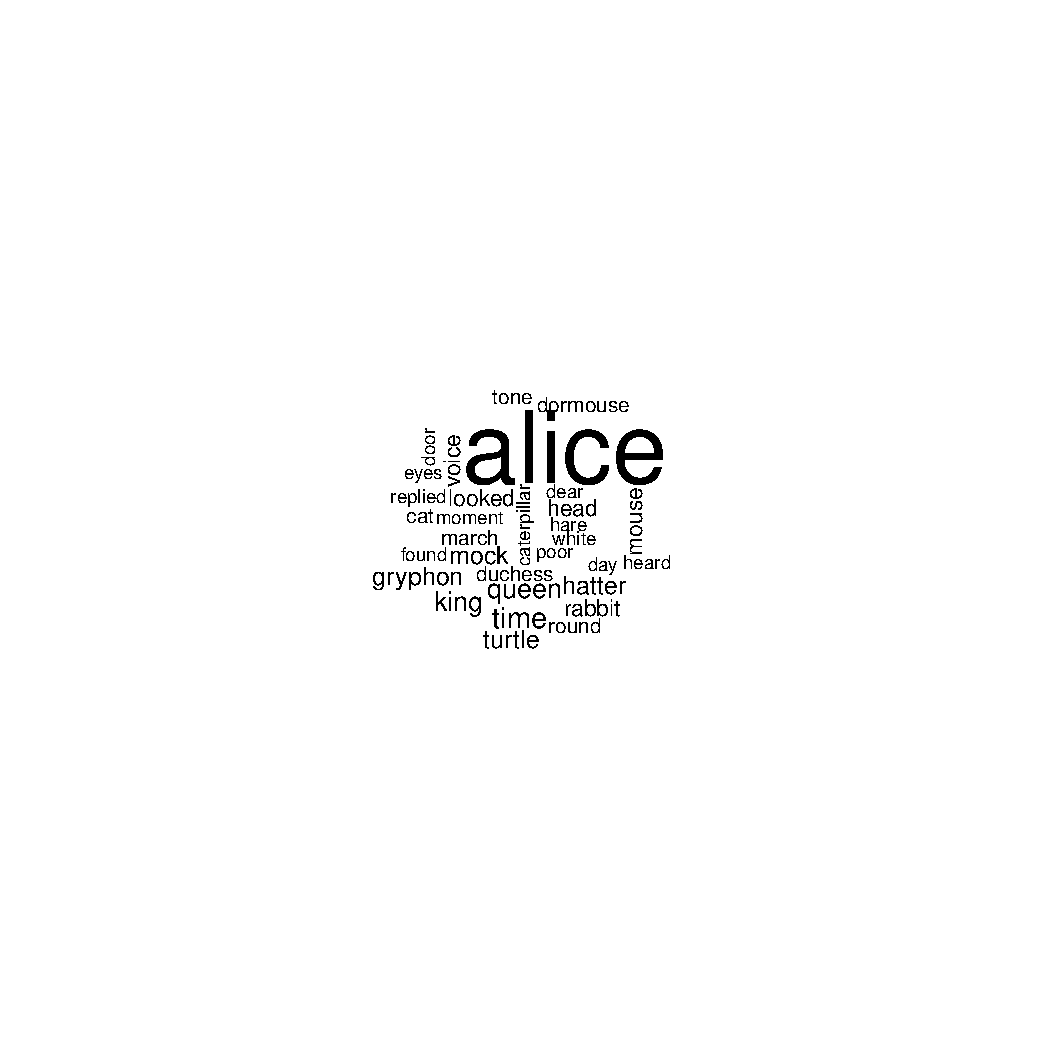
\includegraphics[width=\maxwidth]{figure/unnamed-chunk-5-1} 

\end{knitrout}


\end{document}
